\documentclass[compress]{beamer}
\usepackage[utf8]{inputenc}
\usepackage{hyperref}

\usepackage{tikz}
\usetikzlibrary{graphs, quotes, arrows.meta, matrix}

\usetheme{default}
\usecolortheme{Nord}
\setbeamertemplate{navigation symbols}{}

\title{Segment Tree}
\subtitle{Lazy propagation}
\author{Lorenzo Ferrari, Davide Bartoli}
\date{\today}

\begin{document}

\begin{frame}
    \maketitle
\end{frame}

\begin{frame}{Table of contents}
  \tableofcontents
\end{frame}

\section{Range update -- point query}
\begin{frame}{Range update -- point query}
    \begin{exampleblock}{Problema}
        Dato un array di $N \leq 200'000$ elementi, supporta le seguenti operazioni:
        \begin{itemize}
            \item aumenta di $x$ gli elementi con indice in $[l, r]$
            \item trova quanto vale l'$i$-esimo elemento
        \end{itemize}
    \end{exampleblock}
    \small{\underline{\url{https://cses.fi/problemset/task/1651}}}
\end{frame}

\begin{frame}{Range update -- point query}
    Fin'ora abbiamo affrontato update su un punto e query su un range: qui la situazione \`e invertita.

    \pause
    Esistono pi\`u modi per affrontare il problema, il pi\`u semplice si basa sulla seguente osservazione
    \begin{block}{Osservazione}
        Ogni query su un range, tocca solo i segmenti toccati dai singoli point-update nel range.
        \pause
        \begin{itemize}
            \item possiamo sfruttare questa propriet\`a per invertire le operazioni
        \end{itemize}
    \end{block}
    \pause
    La funzione \texttt{update} assomiglia alla precedente funzione \texttt{query}, la funzione \texttt{query} assomiglia alla precedente funzione \texttt{update}.
\end{frame}

\begin{frame}{Query iterativa}
    \makebox[\textwidth]{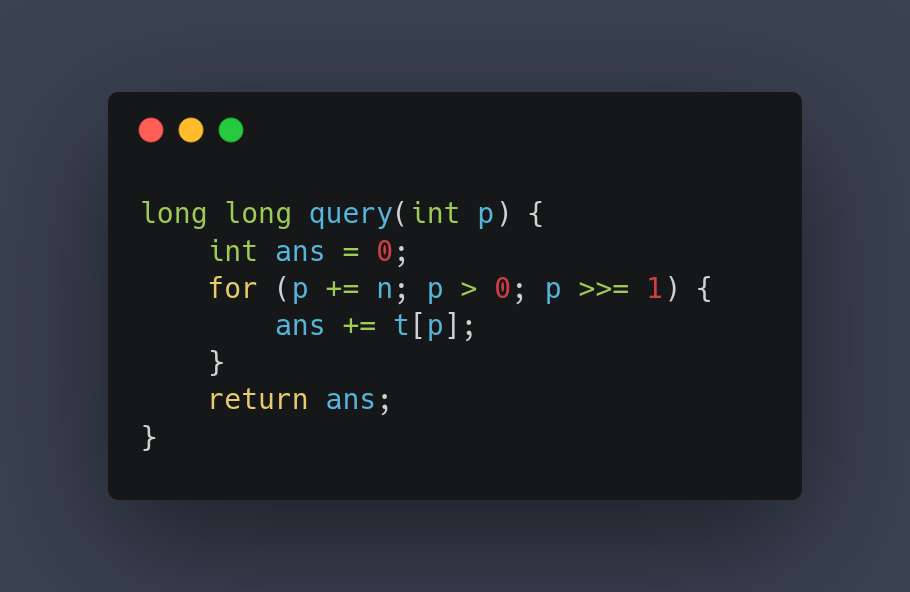
\includegraphics[scale=.3]{./img/seg_qry_it.png}}
\end{frame}

\begin{frame}{Query ricorsiva}
    \makebox[\textwidth]{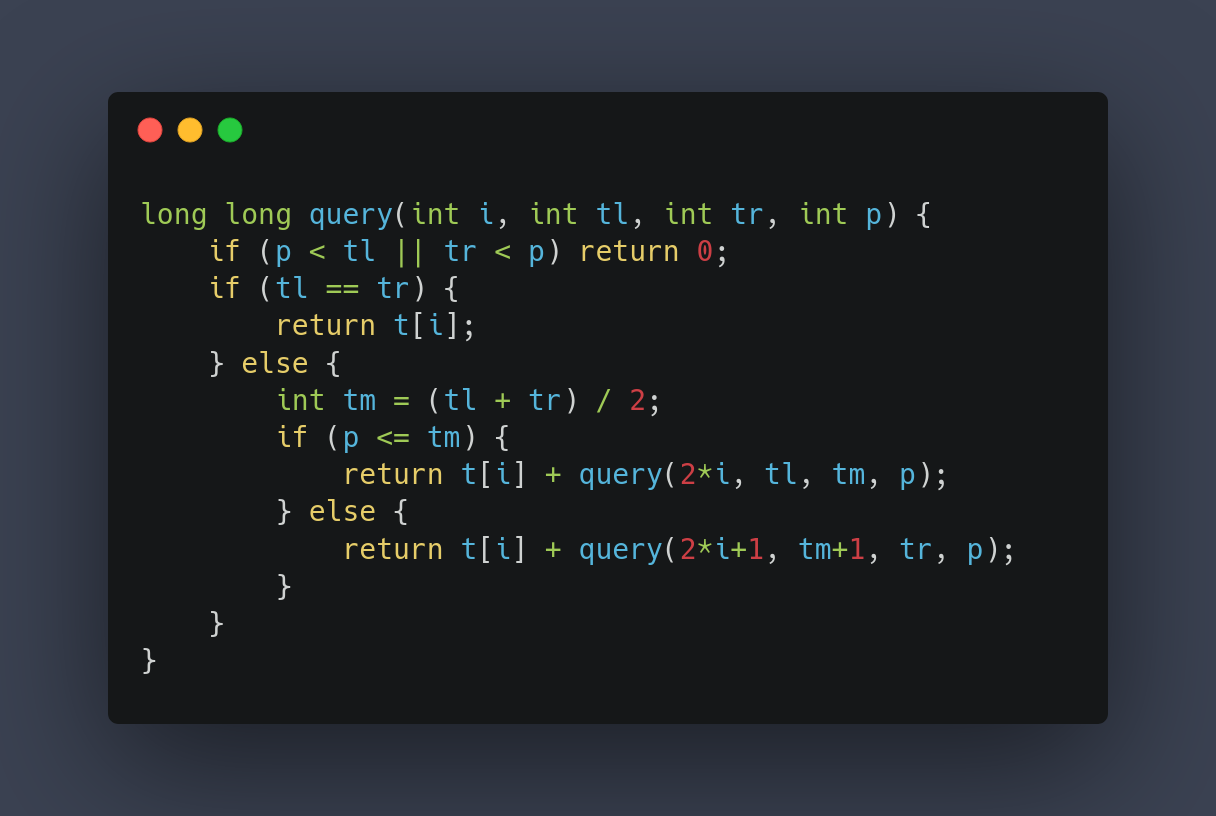
\includegraphics[scale=.3]{./img/seg_qry_rec.png}}
\end{frame}

\begin{frame}{}
    \makebox[\textwidth]{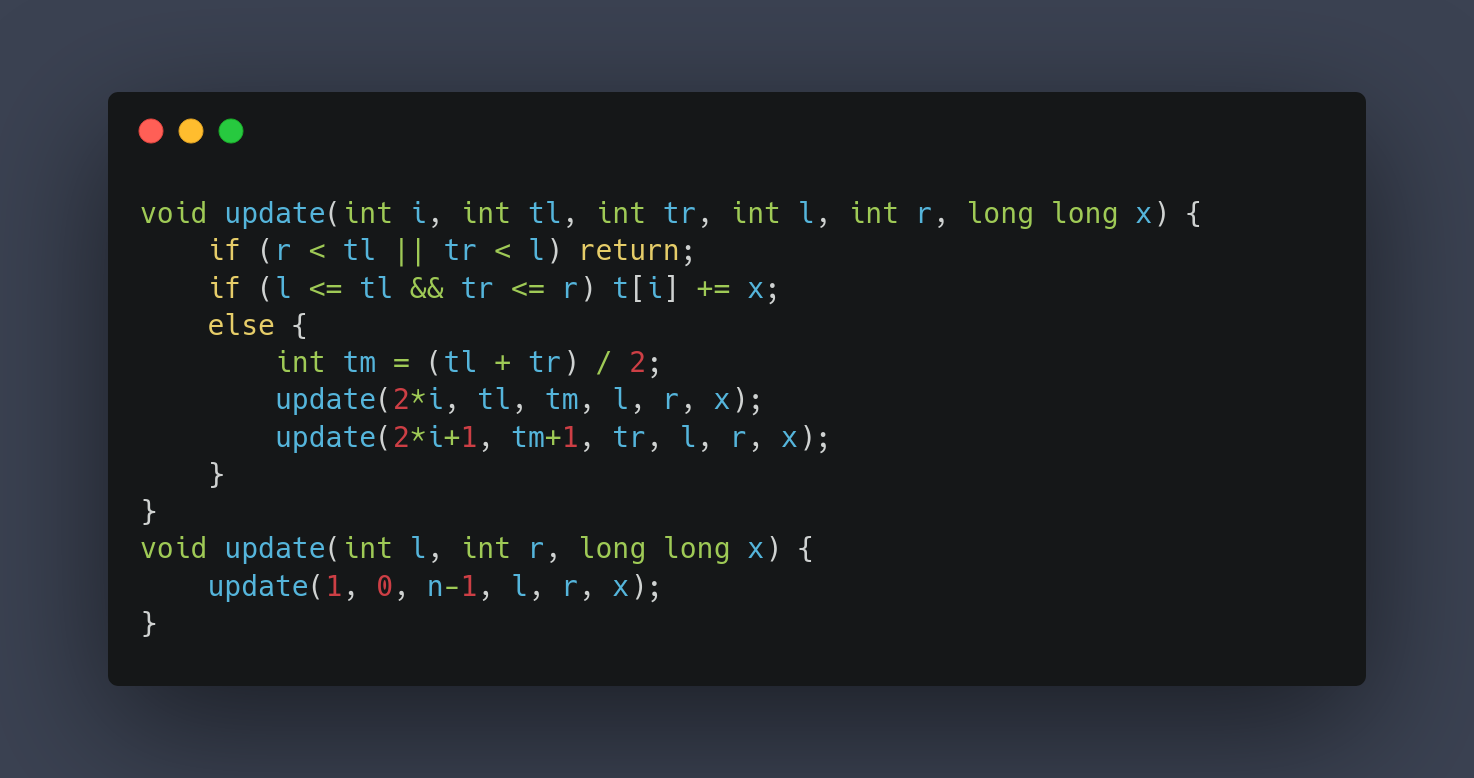
\includegraphics[scale=.25]{./img/seg_update.png}}
\end{frame}

\section{Lazy propagation}

\begin{frame}{Lazy propagation}{Problema}
    \begin{exampleblock}{Lazy propagation}
        Dato un array di $N$ numeri, rispondi alle seguenti query:
        \begin{itemize}
            \item aggiungi $k$ a tutti gli elementi dell'intervallo $[a, b]$
            \item calcola la somma massima di un sottoarray di un intervallo $[l, r]$
        \end{itemize}
    \end{exampleblock}
    Il problema ricorda quello visto nella prima lezione sul segment tree, ma questa volta dobbiamo 
    aggiornare più elementi contemporaneamente.
\end{frame}

\begin{frame}{Lazy propagation}{Idea}
    Potremmo chiamare l'algoritmo visto nella prima lezione $b-a+1$ volte per ogni update, ma ovviamente questo 
    sarebbe troppo lento.\\
    \pause
    Ora l'update è su un range come era la query, quindi possiamo riutilizzare la stessa idea:
    \begin{itemize}
        \item facciamo una dfs per scomporre l'intervallo in un insieme di nodi che formano il nostro intervallo $[a,b]$
    \end{itemize}
    \vfill
    \makebox[\textwidth]{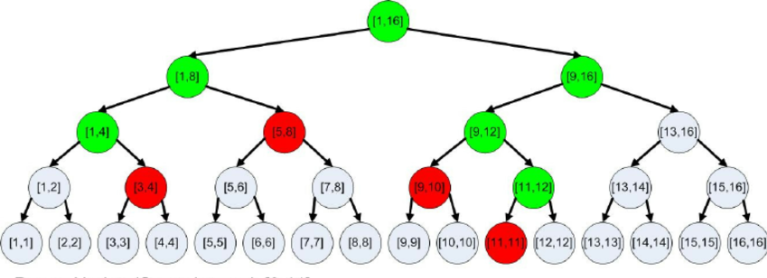
\includegraphics[scale=.30]{./img/query.png}}
\end{frame}

\begin{frame}{Lazy propagation}{Idea}
    Come facciamo ad aggiornare questi nodi dell'albero?\\
    \pause
    Possiamo tenerci un nuovo campo \texttt{aggiungi} che tiene traccia di quanto abbiamo aggiunto agli elementi 
    che sono sotto questo nodo.\\
    \pause
    In questo modo possiamo semplicemente aggiornare il campo \texttt{aggiungi} e fermarci.\\
    \pause
    Ora però le nostre informazioni sono "sparse" tra i nodi dell'albero, e dobbiamo capire come recuperarle per rispondere 
    alle query.\\
    \pause
    L'idea è che ogni volta che visitiamo un nodo, propaghiamo le informazioni di aggiunta verso i nodi figli.\\
    \pause
    Così facendo le informazioni sono sempre aggiornate e possiamo rispondere alle query come prima.\\
    \pause
    La complessità rimane $O(\log n)$ per ogni query e update.
\end{frame}
\begin{frame}{}
    \makebox[\textwidth]{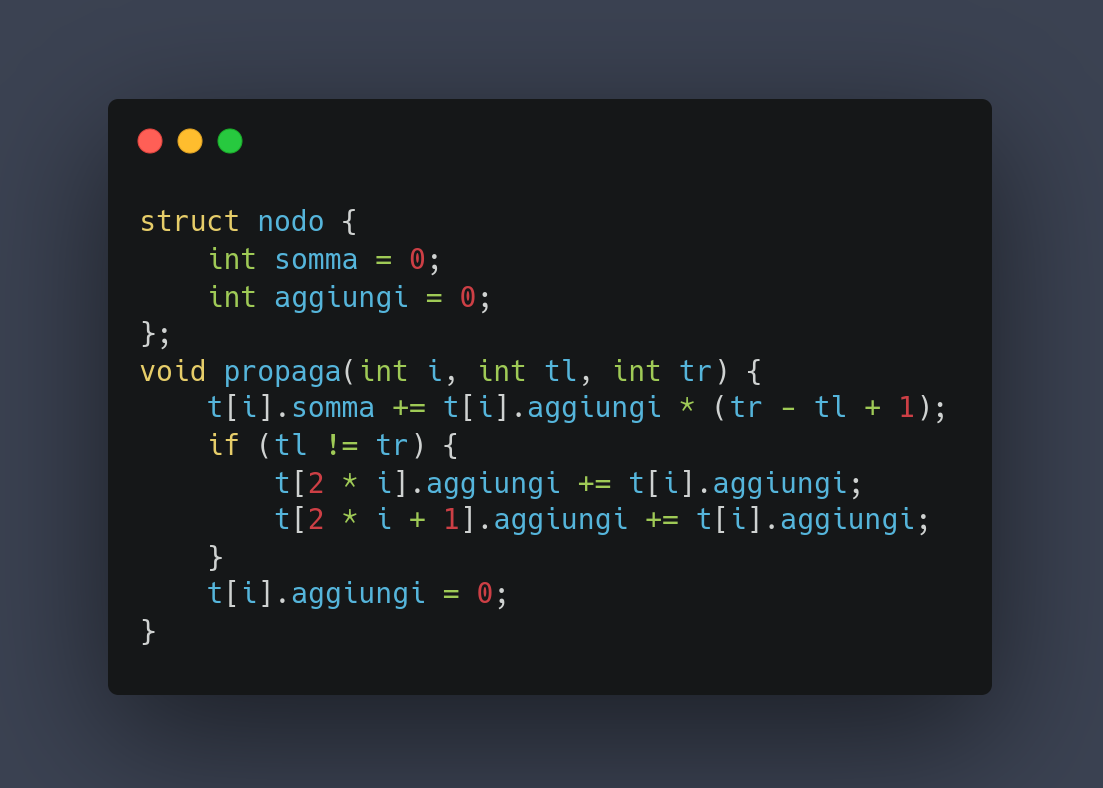
\includegraphics[scale=.30]{./img/lazy_propaga.png}}
\end{frame}

\begin{frame}{}
    \makebox[\textwidth]{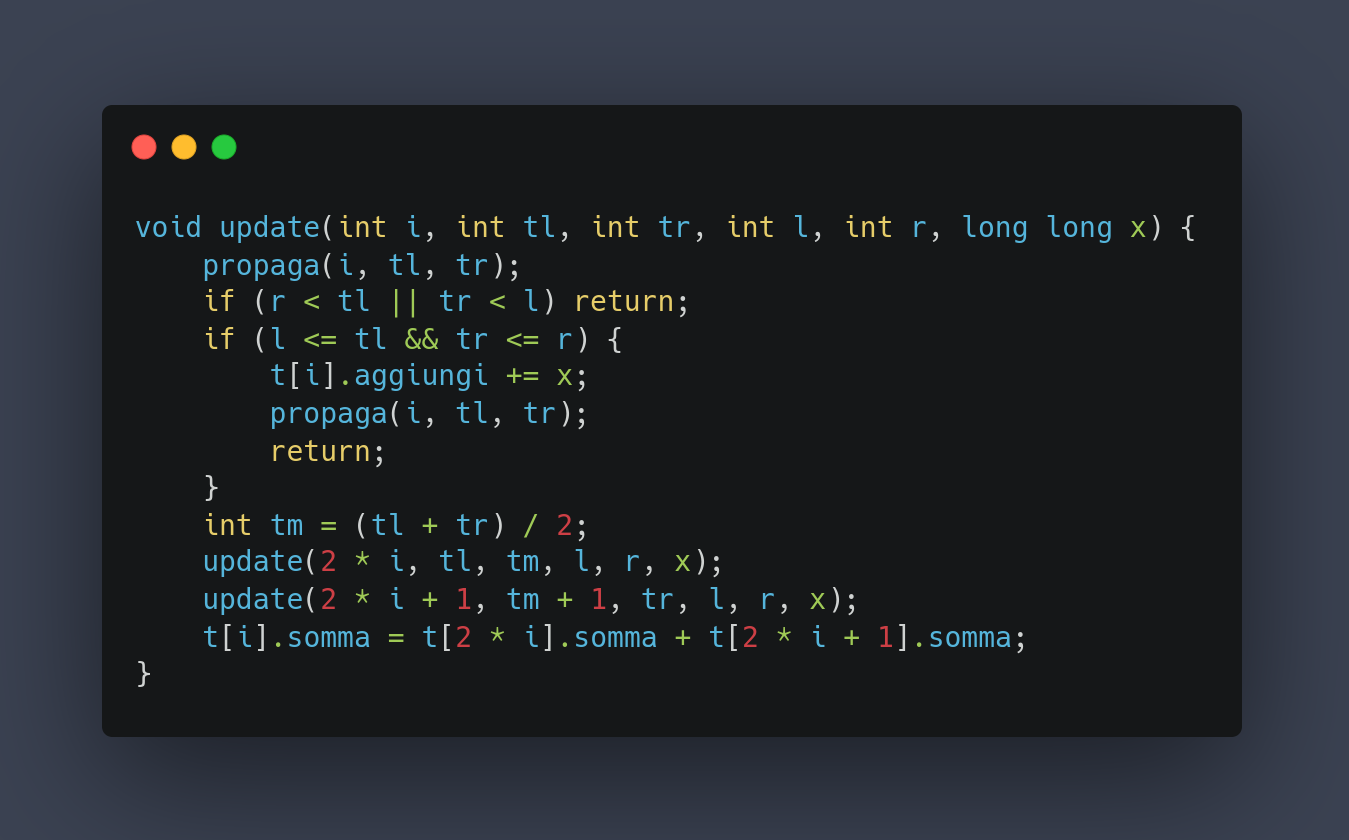
\includegraphics[scale=.25]{./img/lazy_upd.png}}
\end{frame}

\begin{frame}{}
    \makebox[\textwidth]{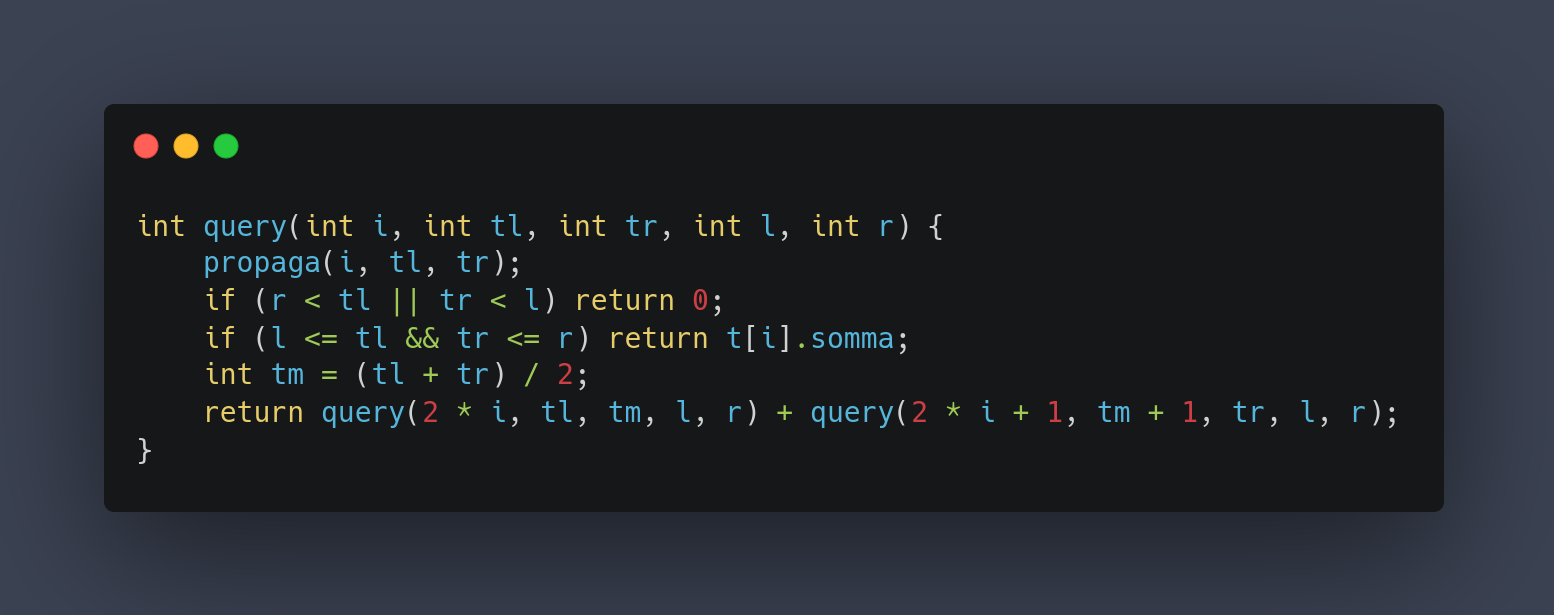
\includegraphics[scale=.25]{./img/lazy_query.png}}
\end{frame}

\begin{frame}{Lazy propagation}{Idea}
    Per poter utilizzare la lazy propagation è necessario poter "unire" 2 query diverse.\\
    In questo caso era semplice, basta sommare i due valori, ma questo non è sempre possibile / a volte 
    richiede alcune accortezze.\\
\end{frame}

\section{Problemi}

\begin{frame}{Problemi}
    \small{\underline{\url{https://cses.fi/problemset/task/1651}}}
    \small{\underline{\url{https://cses.fi/problemset/task/1734}}}
    \small{\underline{\url{https://cses.fi/problemset/task/1735}}}
    \small{\underline{\url{https://cses.fi/problemset/task/1736}}}
    \small{\underline{\url{https://training.olinfo.it/\#/task/segtree/statement}}}
    \small{\underline{\url{https://training.olinfo.it/\#/task/rangetree1/statement}}}
    \small{\underline{\url{https://training.olinfo.it/\#/task/rangetree2/statement}}}
    \small{\underline{\url{https://training.olinfo.it/\#/task/rangetree3/statement}}}
    \small{\underline{\url{https://training.olinfo.it/\#/task/ois_renovations/statement}}}
    \small{\underline{\url{https://training.olinfo.it/\#/task/ois_elevator/statement}}}
\end{frame}

\end{document}
